\documentclass[a4paper,10pt]{article}

\usepackage{fancyhdr}
\usepackage{graphicx}
\usepackage{geometry}
\geometry{a4paper, left=2cm, right=2cm, top=1.5cm, bottom=3cm }
\usepackage{caption}
\usepackage{subcaption}
\usepackage{hyperref}
\usepackage{natbib}
\usepackage{xcolor}
\usepackage{listings}
\usepackage{color}
\documentclass{article}
\usepackage{url}
  \let\oldurl\url
\usepackage{hyperref}
  \let\linkurl\url
  \let\url\oldurl

\definecolor{dkgreen}{rgb}{0,0.6,0}
\definecolor{gray}{rgb}{0.5,0.5,0.5}
\definecolor{mauve}{rgb}{0.58,0,0.82}

\lstset{frame=tb,
  language=Java,
  aboveskip=3mm,
  belowskip=3mm,
  showstringspaces=false,
  columns=flexible,
  basicstyle={\small\ttfamily},
  numbers=none,
  numberstyle=\tiny\color{gray},
  keywordstyle=\color{black},
  commentstyle=\color{dkgreen},
  stringstyle=\color{mauve},
  breaklines=true,
  breakatwhitespace=true,
  tabsize=3
}

\definecolor{sap}{HTML}{822434}


\usepackage{etoolbox,fancyhdr,xcolor}
\newcommand{\headrulecolor}[1]{\patchcmd{\headrule}{\hrule}{\color{#1}\hrule}{}{}}
\newcommand{\footrulecolor}[1]{\patchcmd{\footrule}{\hrule}{\color{#1}\hrule}{}{}}
\renewcommand{\headrulewidth}{1pt}
\headrulecolor{sap!100}%
\renewcommand{\footrulewidth}{1pt}
\footrulecolor{sap!100}%

\fancyhf{}
\fancyhead[R]{
\includegraphics[width=0.25\textwidth]{./figures/logo.png}}

\fancyfoot[L]{Review N.1}
\fancyfoot[C]{Human \& Computer Interaction}
\fancyfoot[R]{\thepage}

\setlength{\headheight}{15mm}
\pagestyle{fancy}

\bibliographystyle{apalike}

\usepackage{times}
\begin{document}

\noindent 
\begin{center}
\textbf{{\Large PAPER TITLE (IN CAPITALS)}} \\
\end{center}

\noindent 
\textbf{Authors: } \textit{L. Scappatura, F. Massaroni, A. Salinetti, L. Ugolini}
\\

\noindent 
\textbf{Advisor: } \textit{Prof. Emanuele Panizzi}
\\

% \noindent 
\textbf{ABSTRACT: } The abstract is a summary of your research project and includes motivation, aims, methods used, (preliminary) findings and (preliminary) conclusions.  The abstract should be a stand-alone document that someone could read to get a general overview of your research project.  

Write the abstract the font shown but make sure it is no longer than about 500 words (and it must fit on a single page which includes the title, authors and keywords). The words of ‘Abstract’ and ‘Keywords’ are set in bold and full caps.  Make sure you put your correct project code in the footer. If you have two supervisors you can list both of them.  If one of them is from industry you should give their company name etc.
Please note the following rules regarding the final paper:
\begin{itemize}
    \item First page (starts with - Title, Authors, Abstract(s) and Keywords) [MANDATORY] and then follows
    \item Body of the paper (text and tables and or figures in the format shown) [MANDATORY]
    \item Notation [OPTIONAL]
    \item Appendices [OPTIONAL]
    \item References [MANDATORY]
\end{itemize}

The total length of the paper is to be no more than \textbf{14pp for 3rdyr and 19pp for 4thyr}. A cover sheet is also required in addition to the research paper. Note that the cover sheet is not included in the page limit.
\\

\noindent 
\textbf{KEYWORDS:} Keyword 1, Keyword 2 and Keyword 3. You can include a maximum of 6 keywords for indexing purposes (spaced by commas). Keywords are single words or short phrases describing the main concepts/topics covered in the paper. Sometimes only 2 or 3 keywords will suffice, but definitely no more than six.
\\

\noindent 
\textbf{STATEMENT OF ORIGINALITY:} Using no more than 8 lines of text (including this one) please give your statement of what is original in this paper. E.g., ‘In this paper a new spreadsheet model is developed to calculate the settlement of foundations making use of previously published methods given by Meyerhof’.
\section{Introduction}
This report provides an overview of all the different phases approached in designing an interface for a fintech application, emphasizing the process of need finding, storyboarding, and prototyping.
It outlines our journey through each phase of the design process, starting with the need finding phase, during which we conducted interviews and gathered insights into users' financial experiences and preferences, leveraging LLMs to have an additional opinion. Subsequently, we moved to the storyboarding phase, where we translated user insights into tangible scenarios and interactions. Finally, we delved into the prototyping phase, where we transformed our conceptual designs into interactive prototypes for usability testing and refinement.
In the whole process, it is highlighted the central importance of incorporating user feedback in the iterative design practices, to end up with a final product reflecting its real-life foundation in the developed features and the design choices. We strived to craft an app interface that does more than just meet basic functionalities. Our approach centered on embracing forefront HCI principles, ensuring the interface both functionality and enjoyability, giving users the possibility to manage their finances gladly and effectively.

\section{Preliminary Need-Finding}
\subsection{LLM Baseline}

With the purpose of gathering valuable information in an efficient way, maintaining an open mind-set not to be occluded by our initial ideas, we needed to formulate questions specific on what we were interested in.\\
Therefore, we first came up with a set of topics and then decided to use an LLM (Large Language Model) to get a preliminary list of possible questions for each of them.




As result of our prompt Fig \ref{fig_prompt} ChatGPT proposed a list of questions we used as a starting point. The questions were too many and sometimes repetitive, so we had to reformulate many of them and reduce redundancies.\\
\begin{figure}[ht]
    \centering
    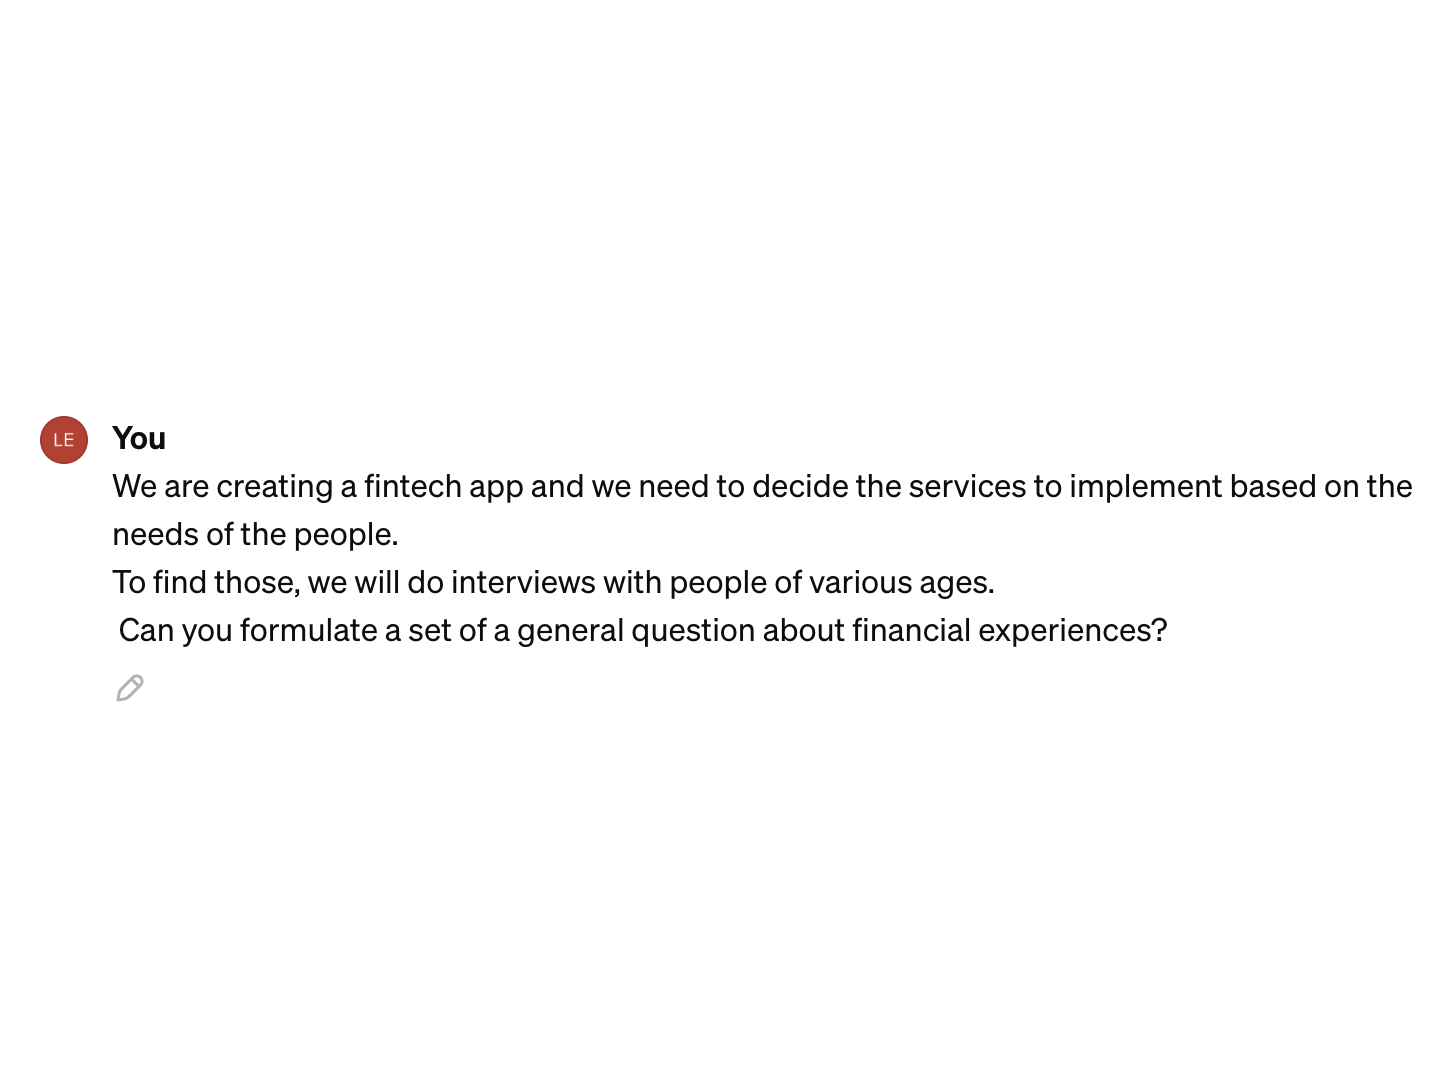
\includegraphics[width=0.5\linewidth]{figures/prompt.png}
    \caption{ChatGPT prompt}
    \label{fig_prompt}
\end{figure}

\subsection{First Interviews}
With questions we considered ready, we approached our first candidate; the result of this first interview taught us two things. First, some questions were obvious or not able to produce useful information; second, they were too many, and contrarily to what expected, the interview lasted about 10 minutes.\\
Fortunately, the interviewee kindly gave us feedback, which was deeply appreciated. We thus needed to further refine and reduce the number of questions, but still ensuring to cover all the macro fields and provide the candidates room to share their experiences.\\
We therefore decided, after refining our questions(available at this \href{https://docs.google.com/document/d/1L25VnXD9_-V7enQ3jEuFU-7WAiuKRug0KEyd9jIrUYU/edit?usp=sharing}{\textbf{link}}), not to propose the whole set of questions to every candidate, but to partition them in batches and ask interviewees only a few of them. In this way, we did not restrict our possibilities of gaining data, and at the same time we reduced the busy time per subject to about 3 minutes.\\
We also opted for asking our chosen LLM also to generate virtual personas and produce answers putting itself in their shoes. LLM's are trained on a big amount of real data, therefore, conceptually, they should be able to represent the average individual for each persona. As expected, it was able to provide reasonable opinions, nevertheless, we still had to gather information from real subjects in order to get a verification or a contradiction.
\subsection{Preliminary Questions Data Analysis}
We had to choose a specific fintech aspect to continue the design process with and the interviews significantly helped us in taking the right decision.\\
We were able to perform in total 20 interviews, and to get a general idea on what people think regarding the proposed topics, we interviewed people around La Sapienza, trying to keep the group as heterogeneous as possible in age, sex, nationality, profession, field of study, place and time.
Some observations from the most recurring responses are the following:\\
Concerning shared expenses, there's a preference for apps like Splitwise or Tricount despite some initial difficulties in using them. It’s not rare to use notes (physical or digital) to keep track of expenses, but this is defined as a suboptimal method, with frequent confusion and mismatch in records; the same problems are encountered when only chat services are used to coordinate.\\
The most utilised payment method is the credit card. Many have successfully experimented with online payments (e.g. PayPal), although some needed to be more intuitive. \\
Lastly, a few practice investing in stocks or cryptocurrencies, utilising specific platforms with benefits and drawbacks. The other interviewees prefer to refrain from investing due to a lack of knowledge or trust.\\
Most are interested in deepening their financial knowledge, and they consider online courses a good resource for this purpose at the expense of face-to-face lessons.
With this information we could discard some of the proposed topics and make some interesting observations on others.
First of all, we excluded investments, cryptocurrencies, blockchain and loans because most people do not know very much on these topics and the few which gave us a positive answer said to already have all the tools needed. Furthermore, we neither have a solid basis to start from, so we did not have enough information to design a relative application.\\
We excluded also cybersecurity, this because interviews did not gave us any evident problem whose solution was suitable for this project.\\
The remaining topics were payments and transactions, personal and shared expenses.
Regarding the first there exist already many affirmed applications which already do this like Paypal or Satispay and we thought that creating a competitor would have been redundant.
Nevertheless, we singled out from multiple interviewees some common problems regarding the management of personal and shared finances:
\begin{itemize}
    \item Lack of awareness in expenses.
    \item Difficulty, also with already existent applications to clearly keep track of a shared fund, and relative problems related to this issue.
\end{itemize}
This gave us a strong clue on a need many people could have, we therefore decided to continue with this track.
\subsection{Study of Competitor Apps}
We studies this, this and this and the problem we found were...\\
After interviews and this study we had a more clear idea on what problems are.
\section{Need Finding on the Specific Topic}
\subsection{Survey on financial habits}
Having this first fairly realistic basis to start with, we could proceed to the next step.
We formulated 
\subsection{Interviews on Financial Habits}
The interviews shed light on various approaches to personal finance management and shared expenses. Most interviewees track their daily expenditures, mostly with banking apps or notes. While the first method is said to reliable, especially when tracking small expenses, the notes method is considered less organised. Others opt not to do so, but some would like to begin.

It was possible to note how the answers given by ChatGPT at the beginning of our need finding process were absolutely not far from the ones given by the interviewed persons, consolidating our assumption in considering both the real and digital personas' answers as reliable.

Based on the responses, we focused on two specific subtopics: tracking expenses and managing shared funds. With these concepts in mind, we developed a questionnaire to reach a broad audience quickly while working on other tasks. To see the questionnaire follow this \href{https://docs.google.com/forms/d/e/1FAIpQLScUr2eKVN_sTKEUXZMMJ9fErrNDnPoO3Dy4FSIO6jOAXINm9Q/viewform}{\textbf{link}}.

\begin{figure}[ht]
     \centering
     \begin{subfigure}[b]{0.45\textwidth}
         \centering
         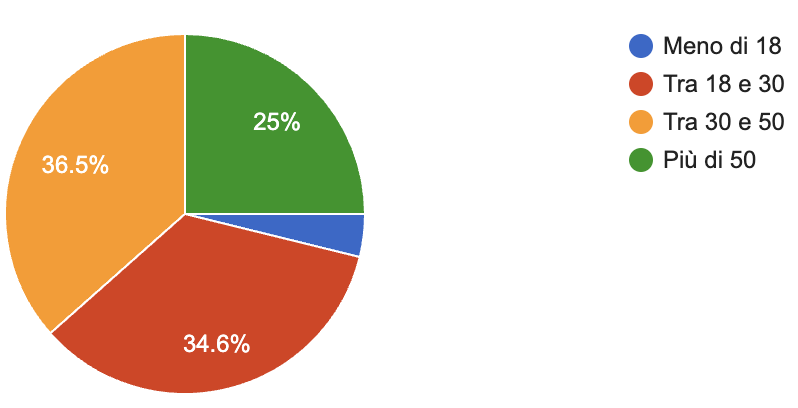
\includegraphics[width=\textwidth]{figures/sexes.png}
         \caption{Age covered}
         \label{fig_age}
     \end{subfigure}
     \hfill
     \begin{subfigure}[b]{0.45\textwidth}
         \centering
         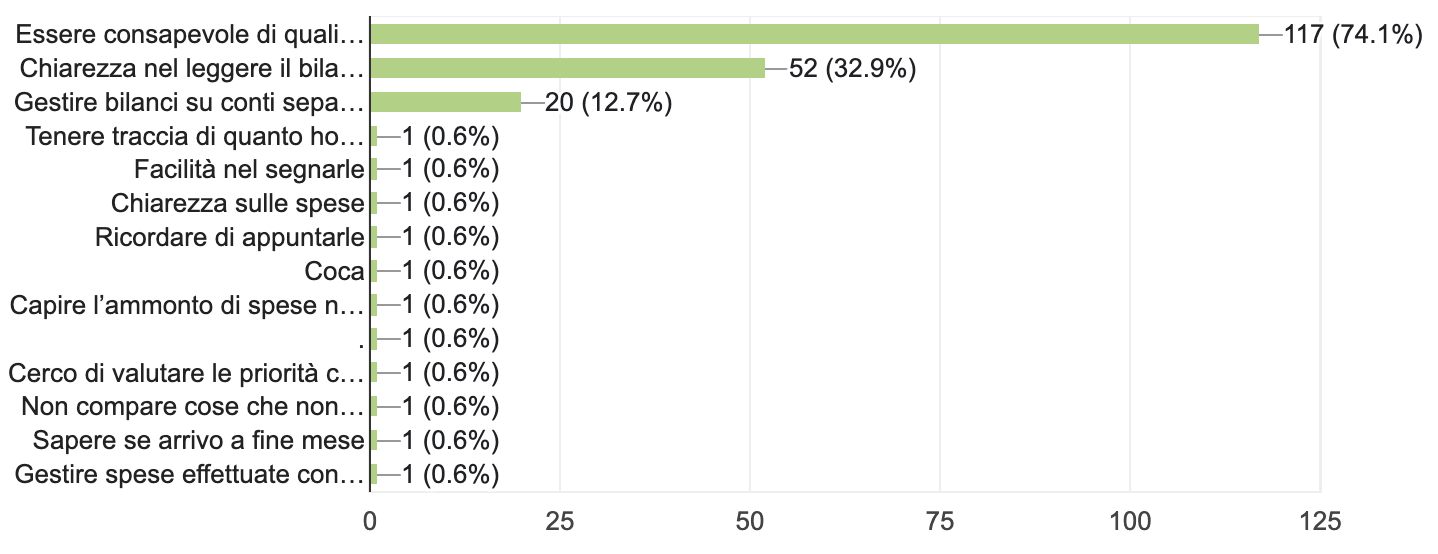
\includegraphics[width=\textwidth]{figures/needs.png}
         \caption{Needs}
         \label{fig_needs}
     \end{subfigure}
        \caption{Age covered (a) and needs (b) were two of the most interesting results}
        \label{fig_results_quest}
\end{figure}

\subsection{Deepening people's needs and features individuation}
The data gleaned from the questionnaire were highly informative and corroborated the needs we initially identified during the first interviews. The participant demographics showed a balanced age distribution Fig.\ref{fig_age}, and importantly, the primary needs expressed in the questionnaire results mirrored those we recognised at the outset Fig.\ref{fig_needs}.$\\$
Despite having initial areas of focus where we would have looked to find the task, we did a second round of interviews based on the questionnaire results. This was to ensure that the needs we identified were truly relevant, so we focused on asking people about their preferences for features involved in money-saver applications. We asked people more specific questions about managing personal and shared finances to understand people's needs.$\\$
Most interviewees stated their need to manage group finances and expenses, evidencing their difficulties. The main problem is the organisation: people lack coordination, causing problems understanding each one’s responsibility for the shared budget or expenses. The availability of a digital service is said to be a possible way to mitigate these situations.
Among the proposed features, two were particularly well-received, sparking inspiration and motivation within our team:$\\$
- Creating a shared fund to prepare a future collective expense, with a step-by-step guide on how and when to collect each personal share.$\\$
- the visualisation of expense records and history$\\$
While the presence of an in-app chat service is redundant, given all the similar services already used, the possibility of in-app payments is considered a good feature, with a little presence of distrust in connecting the personal bank fund/credit card.
\section{Storyboard}
\subsection{The storyboarding process}
In this section, we delve into our storyboarding process, where we started transforming user insights and feedback into visual narratives.  These storyboards serve as a visual roadmap, presenting the features we chose to implement, aligned with user needs and preferences. These sketches are the first representations of the direction we intend for our project to take.
% \section{NEXT HEADING}
Table \ref{tab_materials} contains something interesting. For tables make sure that you use 8 point Times New Roman for ALL the text in the Tables (apart from the caption). Please be consistent throughout your manuscript. Leave one blank line before the table title, another blank line after the title and one blank line after the table. Table titles must be above the table. As with figures the use of color is acceptable in tables. Make sure that the table does not run across multiple pages. If it does then have a repeat of the table caption with the word ‘continued’ in brackets after it.


\begin{table}[h]
\begin{center}
\caption{Summary of the database (note that table captions go ABOVE THE TABLE)}
\begin{tabular}{ |l|c|l| }
\hline
 \textbf{Column heading} & \textbf{Column heading}    & \textbf{Column heading} \\ \hline 
 Table Text     & 10     & Falling head permeameter \\  \hline 
 Concrete       & 2      & Strong \\ \hline 
 Steel          & 1      & Stronger \\ \hline 
 Timber         & 3      & Weak \\ 
 \hline
\end{tabular}
\label{tab_materials}
\end{center}
\end{table}

% \section{SUMMARY}
The conclusions to be drawn from this work are as follows:
\begin{itemize}
    \item 	This is a great template
\end{itemize}


At the end of the reference list no more than 15 pages should be in your ENTIRE document (including the cover sheet). Do check else a penalty will be applied!  (For students enrolled in CENGM0080 your document including the cover sheet must be no longer than 20 pages using this template).

Remember you need to submit your research paper as a PDF document! Make sure you check that all the fonts, figures and text is preserved in the layout you intend when PDF conversion is done!


\subsection{Limitations and Recommendations for further work}

For this research paper it is useful to include this section where you discuss the limitations of your work and point to future work.
% \section{ACKNOWLEDGEMENTS}
Use this section to thank people who have assisted during the project – if you want. It is good form to thank your supervisor, technicians and doctoral students who have helped and anyone else who deserves a mention – but do not make it too personal. 

For example, ‘the author wishes to thank Dr X for their supervision throughout the year and also Mr G who helped build the testing rig described in this paper.’
Use this section to thank your data sources including citations to the data, weblinks, etc.
% \section{APPENDIX I}
These are NOT RECOMMENDED. However, if you want to put a mathematical derivation or large data table at the back of the paper in an appendix please put it before the NOTATION LIST. 
% \section{APPENDIX II}
If a second appendix is used then call the first appendix ‘APPENDIX I’ and the second ‘APPENDIX II’ and so on.
% \section{NOTATION}
This section is optional. If you have few equations it may be better to simply define all the variables in the text as shown. For highly mathematical papers this section is very helpful for the reader. Note that this section heading is not numbered. Please put the following statement in italics before the notation list:

\textit{The following acronyms and symbols are used in the work described in this paper:}

\textbf{Acronyms}

BSI	 British Standards Institute

\textbf{Symbols}

\textit{Latin}

$A$ = a constant

\textit{Greek}

$\gamma$ = shear strain

\fontsize{8}{9}\selectfont


\bibliography{ResearchPaperBib}



\clearpage



\end{document}